\chapter{Introduction} \label{chap:Introduction}

\section{Zoonoses and the risks of pandemics}

In times where infectious disease outbreaks become more frequent and sometimes even reach global appearance, unpredictable effects on humans, wildlife and whole ecosystems are inevitable \autocite{schmeller_biodiversity_2020}. Growing human population and persisting poverty has harmful impact on the biodiversity and results in degradation of natural habitats and more frequent human-wildlife contacts  \autocite{schmeller_biodiversity_2020}. Therefore, increasing numbers of zoonoses, transfers of animal pathogens on humans, arise and are a major driving force in pathogen emergence on humans in recent decades \autocite{jones_global_2008}. Most of the human pathogens emerging lately are of animal origin, indeed, up to 75\% \autocite{woolhouse_risk_2001}. Well-known examples of zoonoses are avian and swine flu \gls{HIV}, ebola, \gls{MERS} and \gls{SARS} including the current circulating COVID-19 \autocite{van_reeth_avian_2007, sharp_origins_2011, suwantarat_risks_2015, verity_estimates_2020}.

While zoonoses can be of viral, bacterial and parasitic nature, emergences of higher magnitude, like the mentioned well-known examples, are often linked back to viral infections \autocite{woolhouse_risk_2001}. Harmfulness of viral infections can be diverse, ranging from mostly no sign of infection in the natural hosts to very severe symptoms or death in accidental hosts \autocite{wahlgren_influenza_2011}. In contrast to natural hosts, humans, accidental hosts to, e.~g.~, the West Nile Virus, develop disease patterns upon infection and, thereby, are not able to support the virus life cycle \autocite{gea-banacloche_west_2004}. High variety in host circulation and transmission ways from such natural or intermediate onto humans as accidental hosts, with long infectious periods without symptoms and high transmission pace have a high risk of pandemic events \autocite{jamison_chapter_2017}. A prominent virus detected in a variety of hosts and known for reoccurring local and global outbreaks in the past is \gls{IAV}, member of the \textit{Orthomyxoviridae} family and also commonly known as flu \autocite{wahlgren_influenza_2011}. Analysis indicate a 1\% chance of a pandemic with millions of deaths every year and is, therefore, the pathogen most likely to be responsible for a sudden severe pandemic \autocite{jamison_chapter_2017}. 

\section{Life-cycle and structure of the \textit{Influenza A Virus}}

\begin{figure}
    \centering
    %\begin{adjustbox}{minipage=\dimexpr\textwidth-2\fboxsep-2\fboxrule,fbox}
    \begin{subfigure}[b]{0.475\textwidth}
        \caption[\textit{Alphainfluenzavirus}]{\textbf{\textit{Alphainfluenzavirus}}}
        \label{subfig:Influenza_A}
        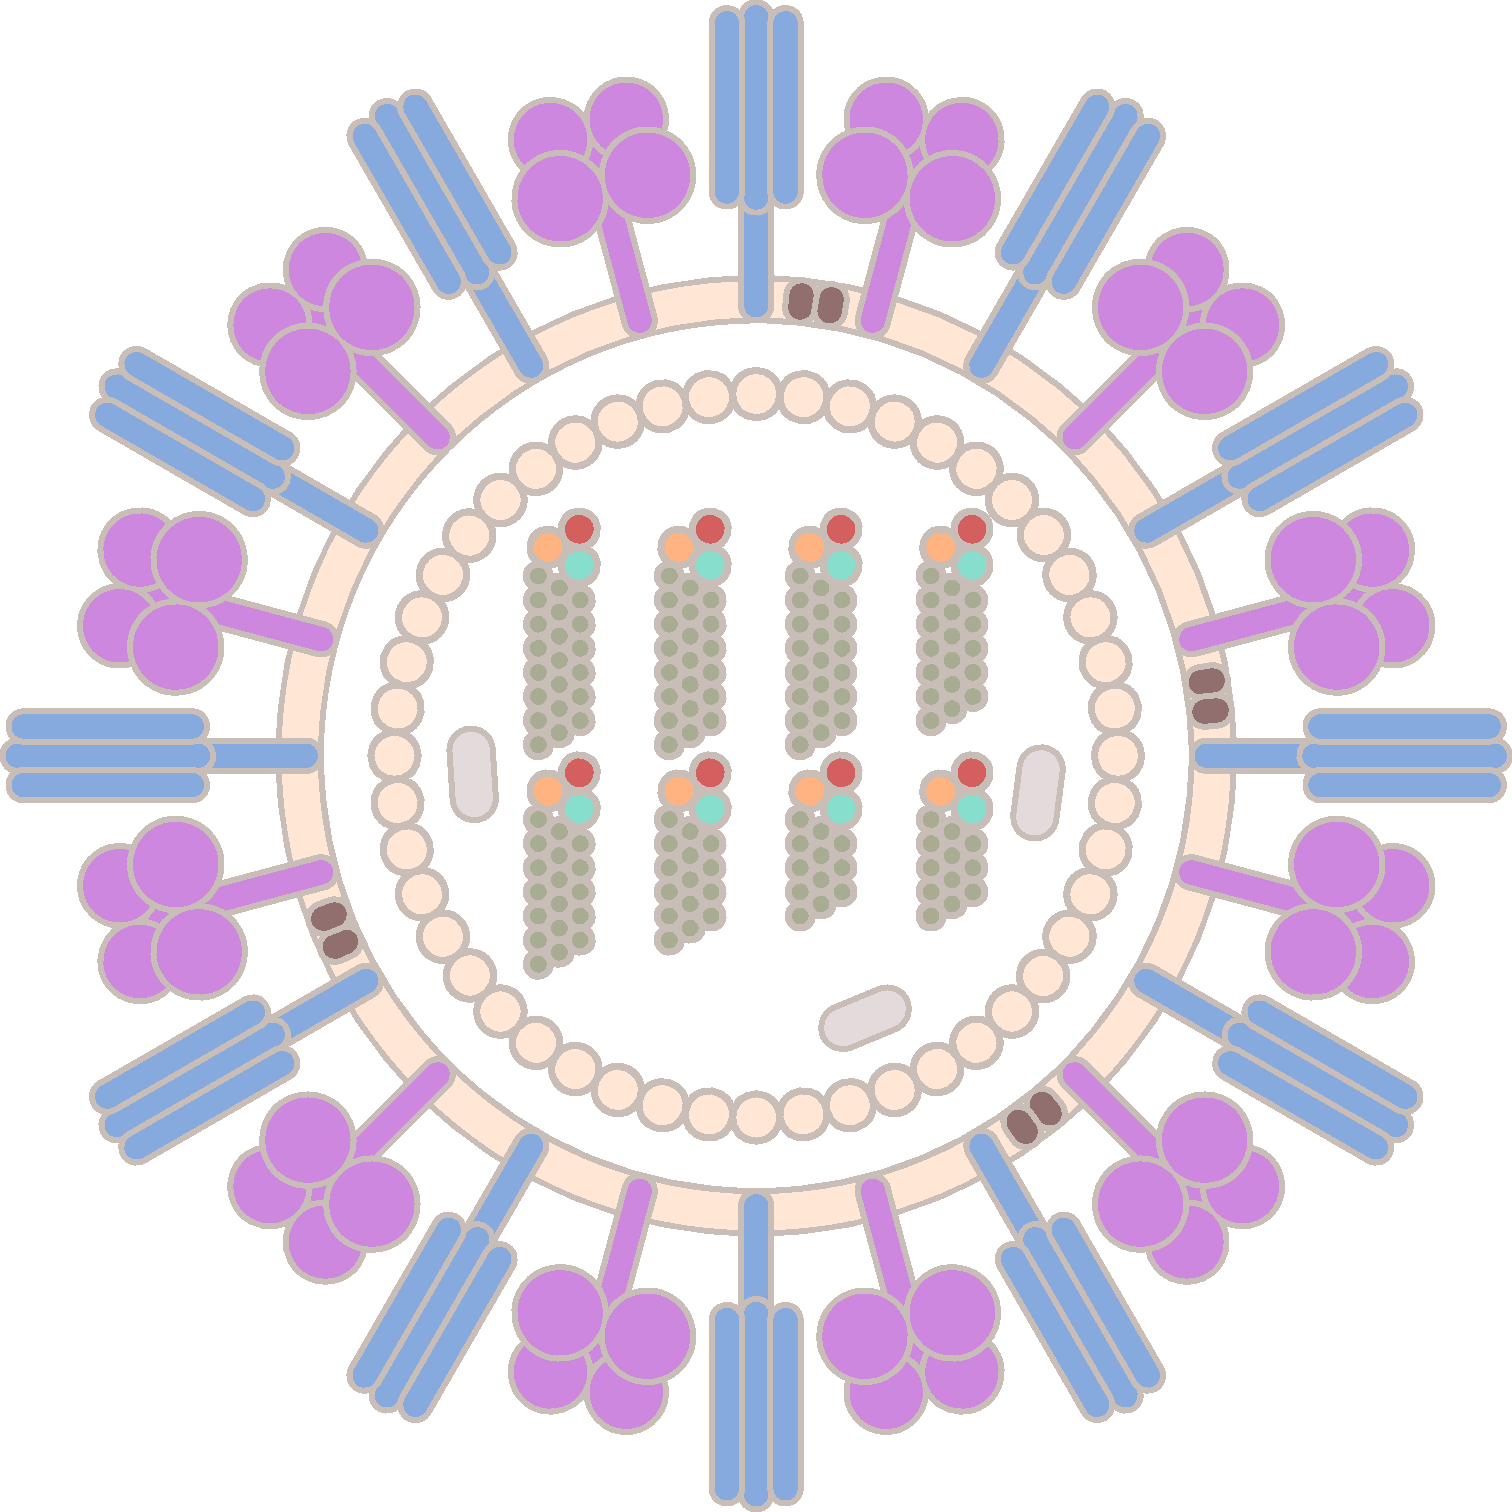
\includegraphics[width=\textwidth]{Graphics/Influenza_A.pdf}
    \end{subfigure}
    \hfill
    \begin{subfigure}[b]{0.475\textwidth}
        \caption[\textit{Betainfluenzavirus}]{\textbf{\textit{Betainfluenzavirus}}}
        \label{subfig:Influenza_B}
        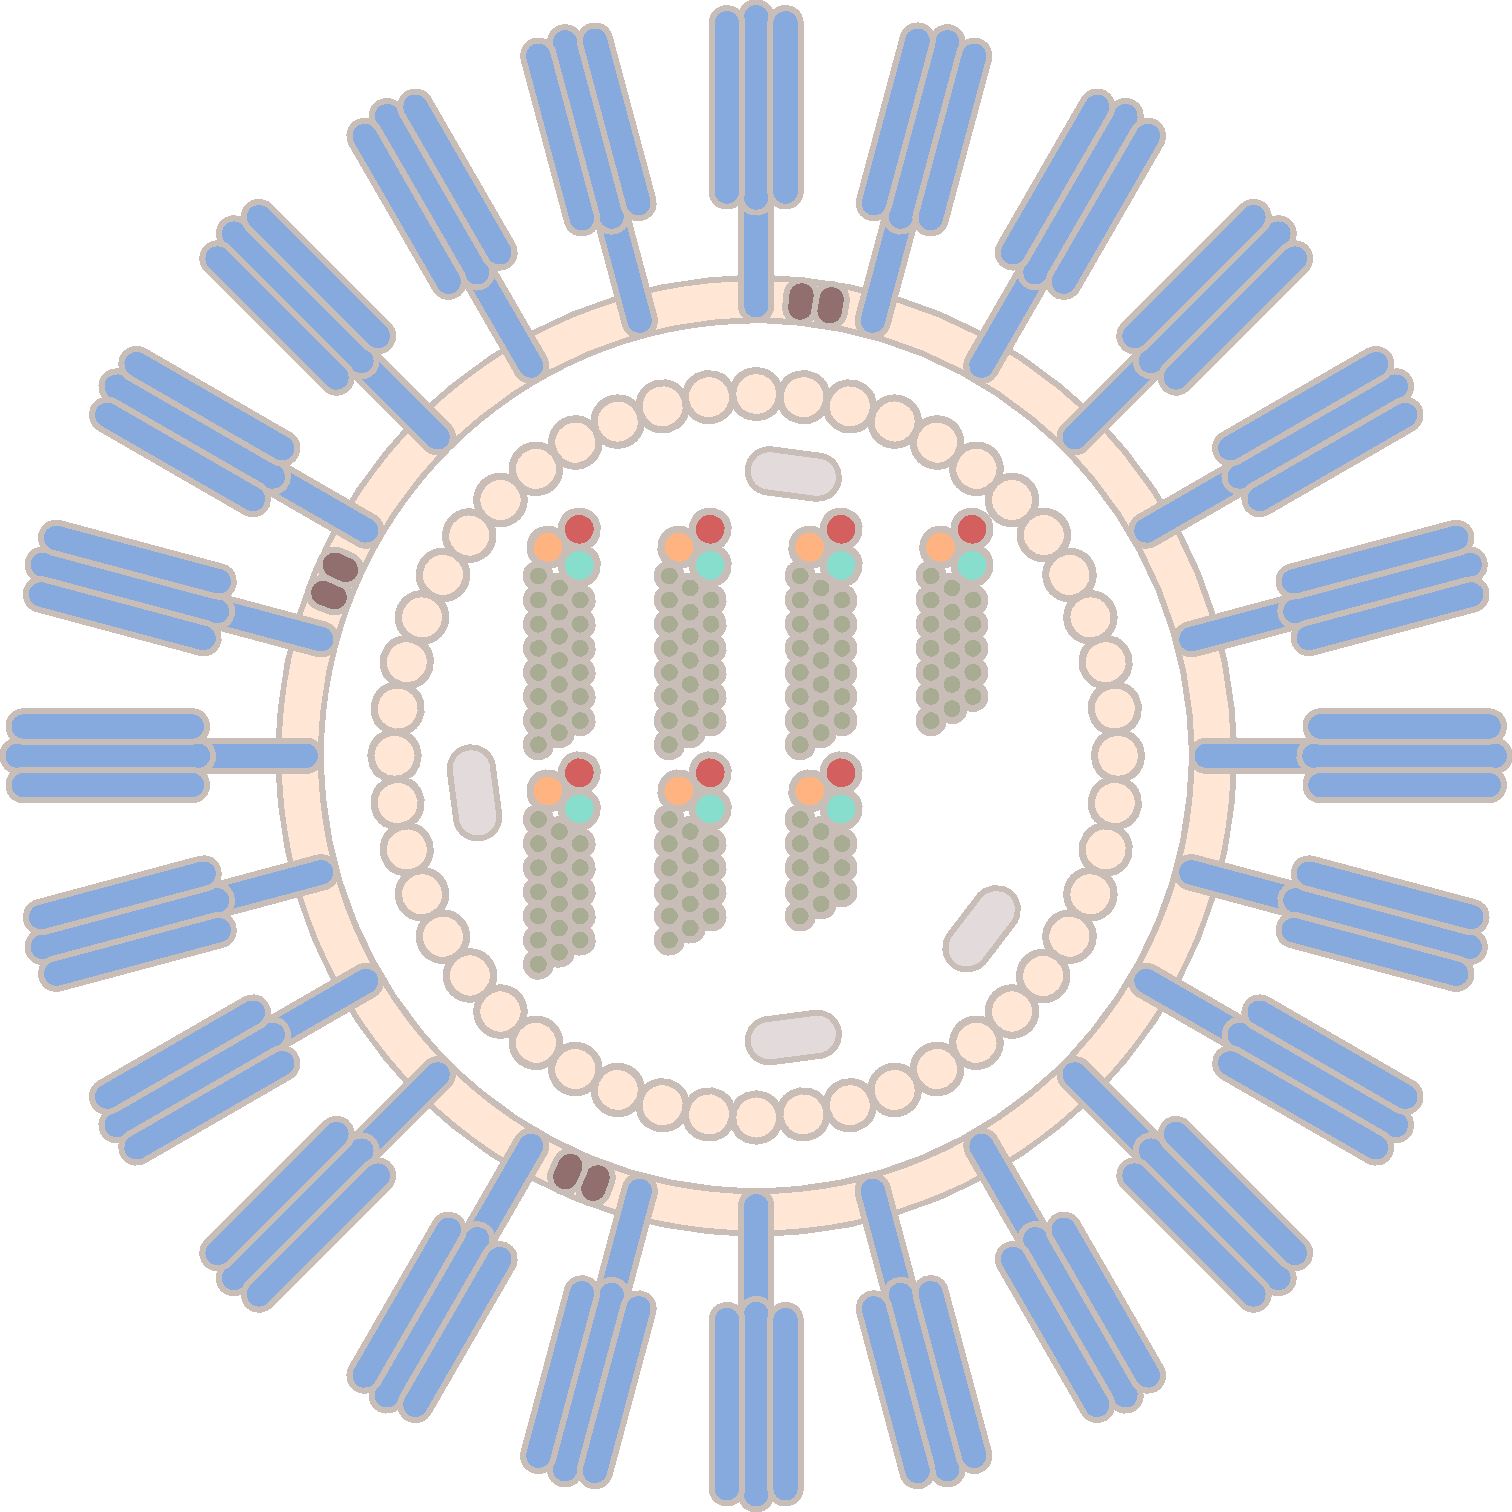
\includegraphics[width=\textwidth]{Graphics/Influenza_B.pdf}
    \end{subfigure}
    %\end{adjustbox}
    \caption[\textit{Orthomyxoviridae}]{\textbf{\textit{Orthomyxoviridae}.} .}
    \label{fig:Orthomyxoviridae}
\end{figure}

In humans, infection by \gls{IAV} affects the upper respiratory tract \autocite{julkunen_inflammatory_2000}. General symptoms like fever, cough and headache characterize the infection \autocite{julkunen_inflammatory_2000}. In some cases complications can occur, resulting in primary viral pneumonia or secondary bacterial pneumonia by bacterial infection \autocite{julkunen_inflammatory_2000}. The virus particles of \gls{IAV}, called virions, are spherical in shape, 80–120nm in size and enveloped by the hosts cell membrane lipids \autocite{oxford_chapter_1987, mudhakir_learning_2009, cann_chapter_2016}. These virions can sustain extensive forces in the hosts body and even survive deformation to around 33\% of the its total diameter \autocite{schaap_effect_2012}. Epithelial cells in the tissue of the respiratory tract, are the main infection area of the virions \autocite{oxford_chapter_1987}. The \gls{IAV} virions attach themselves to the host cells with their surface glycoproteins, the tetrameric \gls{NA} and the trimeric \gls{HA} and enter the cells by clathrin-mediated endocytosis (\autoref{subfig:Influenza_A}) \autocite{wilson_structure_1981, varghese_structure_1983, jones_global_2008, mudhakir_learning_2009}. Equilibration of pH in the process of endocytosis involve the transmembrane protein \gls{M2} of \gls{IAV} \autocite{pielak_influenza_2011}. The surface glycoprotein tails are also connected to the second layer in the \gls{IAV} virions, the \gls{M1} \autocite{ali_influenza_2000}. Following the endocytosis the \gls{RNP} complexes are carried to the hosts cells nucleus by \gls{NPC} for virus replication \autocite{eisfeld_at_2015}. These \gls{RNP} complexes contain the viral \gls{ssRNA}, holding the genetic information, bound to multiple \glspl{NP} and the polymerase complex \autocite{eisfeld_at_2015}. The trimeric polymerase complex including the \gls{PB1}, \gls{PB2} and \gls{PA} is essential for viral replication in the hosts nucleus \autocite{area_3d_2004, eisfeld_at_2015}. \gls{IAV} is a segmented virus, one virion of \gls{IAV} contains eight different short \glspl{ssRNA}, called segments, encoding in total 14 viral proteins \autocite{eisfeld_at_2015}. In the nucleus the eight \glspl{ssRNA} are replicated and transcribed to \glspl{mRNA} with the latter translated to the virions proteins in the cytoplasm \autocite{eisfeld_at_2015}. The translated \gls{NEP}, \gls{M1}, \gls{NP} and proteins of the polymerase complex are imported by the \gls{NPC} to build new \glspl{RNP} with the replicated genomes and enable the nuclear exit \autocite{eisfeld_at_2015}. By budding through the plasma membrane with the translated \gls{M2}, while incorporating the translated \gls{HA} and \gls{NA} into the surface, new virions are released \autocite{eisfeld_at_2015}.

\section{Evolution of the \textit{Influenza A Virus}}

Present day research, indicate mallards \textit{(Anas platyrhynchos)} as main reservoir and natural host of \glspl{LPAIV} \autocite{jourdain_influenza_2010}. Studies on Pekin ducks, descended from mallards, have shown minor immune responses and antibody production to the infection with \gls{IAV} strains and the possibility of a reinfection after two months with the same strain \autocite{kida_duck_1980}. Strains are lines of \gls{IAV} related to a specific location and time point \autocite{cann_chapter_2016}. Less dangerous strains of \gls{IAV}, called \glspl{LPAIV}, seem to repeatedly circulate in duck species and may evolve into human pathogenic strains by zoonoses \autocite{jourdain_influenza_2010}. Simple transmission over species is not enough to start a pandemic though, therefore, better understanding of the mostly unknown genetic changes vital for zoonotic events is required \autocite{van_reeth_avian_2007}. Circulation of these strains in aquatic bird species with continued evolution enable the transmission possibilities to humans, lower animals, and other birds \autocite{webster_chapter_1999}. The evolution occurs in all segments of the \gls{IAV} but is most prominent in \gls{HA} and \gls{NA} \autocite{webster_chapter_1999}. Infection is mostly dependent on these surface glycoproteins, building the serotype, of the virus, as they are crucial for attachment to host cells \autocite{cann_chapter_2016}. Significant variation in the surface glycoproteins mostly occur by reassortment, also called genetic shift and point mutations, also called antigenic drift \autocite{webster_chapter_1999}. 

Point mutations in the segmented genome are very frequent, as the mutation rate in all RNA viruses is very high \autocite{duffy_why_2018}. Present \textit{poliovirus} research, indicate higher selection for faster replication and, therefore, acceptance of replication errors in favor of faster viral polymerases \autocite{pfeiffer_increased_2005, duffy_why_2018}. This finding is in line with research indicating the short length or segmentation of RNA viruses and the high mutation rates as evolutionary trade-off \autocite{belshaw_pacing_2008, vignuzzi_closing_2012}. Thereby, creating a cloud of offsprings, called quasispecies, with 1-2 mutations in the genome each \autocite{belshaw_pacing_2008, vignuzzi_closing_2012}. The point mutations affect the offsprings surface proteins \gls{AA} composition in the translation process, by possible missense and nonsense errors or frameshifts \autocite{parker_errors_1989, webster_chapter_1999}. Reassortment is a more drastical change in the surface proteins and likely to be related to the pasts most horrible \gls{IAV} pandemic, the spanish flu in 1918 \autocite{nelson_multiple_2008}. For reassortment induced zoonoses, there has to be a intermediate host or \glqq mixing vessel\grqq{}, most likely pigs, able to be infected by \glspl{IAV} of different hosts \autocite{shu_evidence_1994}. The hosts cells can then be co-infected by two different \glspl{IAV} and create offsprings with mixed segments \autocite{compans_influenza_2014}. All segments can be exchanged, but, in case of surface proteins of different hosts, \glspl{IAV} can occur that are able to do interspecies transmission \autocite{shu_evidence_1994}. Avian \gls{IAV} strains can, thereby, evolve to human strains by co-infection of a pig with human transferable and avian originating \gls{IAV} strains \autocite{shu_evidence_1994}. 

\section{Vaccines design and the link to reassortment}

No real cure to \gls{IAV} infection is available and generation of vaccines is straining and not always as effective as expected \autocite{wahlgren_influenza_2011, wong_traditional_2013}. Furthermore, the efficacy of vaccines vary in specific populations and there are limitations to the manufacturing and the time frame of the production \autocite{wong_traditional_2013}. The strains most likely to circulate for the season are selected twice a year by the \gls{WHO}, to be included in vaccines prepared for the winters in both hemispheres \autocite{barr_epidemiological_2010}. The seasonal used \gls{IAV} vaccines target the highly mutable head domain of \gls{HA} surface proteins to stimulate immune response \autocite{wong_traditional_2013, wei_next-generation_2020}. Therefore, the \gls{IAV} vaccines efficiency vary depending on the similarity of the \gls{HA} head domain of the strains used for the vaccines and the ones circulating in the season \autocite{wei_next-generation_2020}. To manufacture the vaccines, reassortment of the selected strain with a master strain is induced in eggs \autocite{wong_traditional_2013}. The resulting hybrid strain contains the selected strains surface proteins and the master strains high-growth properties necessary for production of the vaccine in the short time frame \autocite{wong_traditional_2013}. Therefore enlarging the knowledge of \gls{IAV} reassortment is important for predicting future pandemic strains, creation of vaccines by high-growth hybrid strains and the overall efficiency of the vaccines against the seasons circulating variable strains \autocite{wong_traditional_2013, dadonaite_structure_2019}. For better understanding of \glspl{IAV} reassortment, the secondary structure of the genome segments and their interaction mechanisms have to be discovered \autocite{dadonaite_structure_2019}. 

\section{Secondary Structures of the \textit{Influenza A Virus}}

The eight \gls{IAV} \gls{ssRNA} segments are single-stranded chains of nucleotides, by inter- and intra-molecular base-pairing various complex arrangements with different stabilities can be build \autocite{higgs_rna_2000, dadonaite_structure_2019}. Negative single-stranded RNA viruses can use secondary structures on the \gls{ssRNA} as well as on the transcribed positive \gls{mRNA} for different mechanisms, like the initiation of the translation on the \gls{mRNA} by the \gls{IRES} or inter-molecular binding of different \gls{ssRNA} segments to each other \autocite{kieft_viral_2008, moss_identification_2011, dadonaite_structure_2019}. Prediction of these viral secondary structures is possible by lab methods \textit{in virio} and \textit{in vitro} or \textit{in silico}, with the latter only based on thermodynamic calculations alone \autocite{moss_identification_2011, dadonaite_structure_2019}. \textit{In virio} methods involve modification inside a virion and \textit{in vitro} methods involve modification on transcribed RNA in a probe, both can used e.~g.~, with SHAPE-MaP \autocite{smola_selective_2015, dadonaite_structure_2019}. Therefore, both methods can only be used to analyze secondary structure folding on single viruses, but reveal structures at single-nucleotide resolution \autocite{dadonaite_structure_2019}. \textit{In silico} methods that are used without support by experiments are not limited by prediction on single viruses, only require prior sequenced genomes \autocite{moss_identification_2011, dadonaite_structure_2019}. Since \textit{in silico} methods can be used on more than one virus, secondary structures can be predicted all together to find conserved equal folding regions in the sequenced genomes with alignments \autocite{moss_identification_2011}. 

\section{Alignments and clustering}

\begin{figure}
    \centering
    %\begin{adjustbox}{minipage=\dimexpr\textwidth-2\fboxsep-2\fboxrule,fbox}
    \begin{subfigure}[b]{0.475\textwidth}
        \caption[Compactness]{\textbf{Compactness}}
        \label{subfig:Compactness}            
        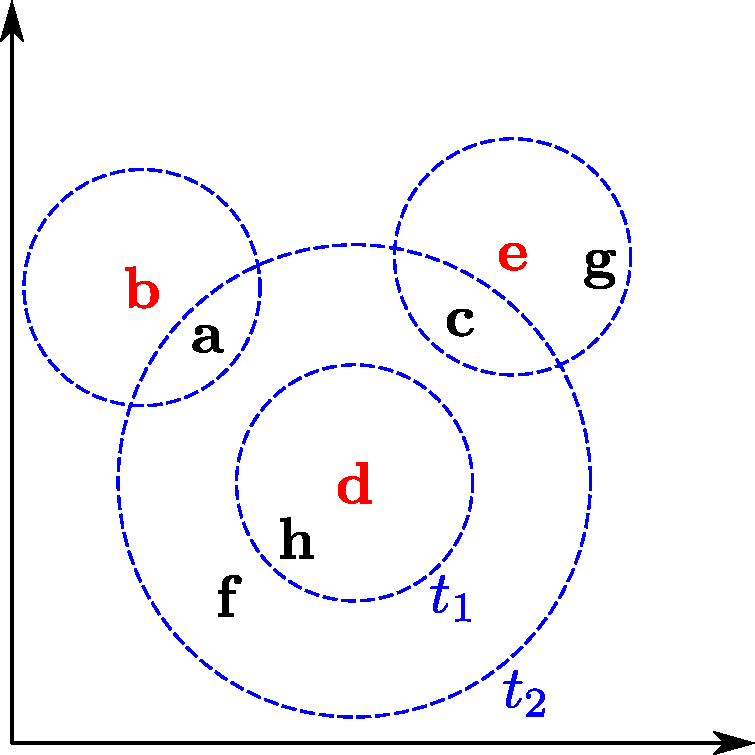
\includegraphics[width=\textwidth]{Graphics/Compactness.pdf}
    \end{subfigure}
    \hfill
    \begin{subfigure}[b]{0.475\textwidth}
        \caption[Connectedness]{\textbf{Connectedness}}
        \label{subfig:Connectedness}            
        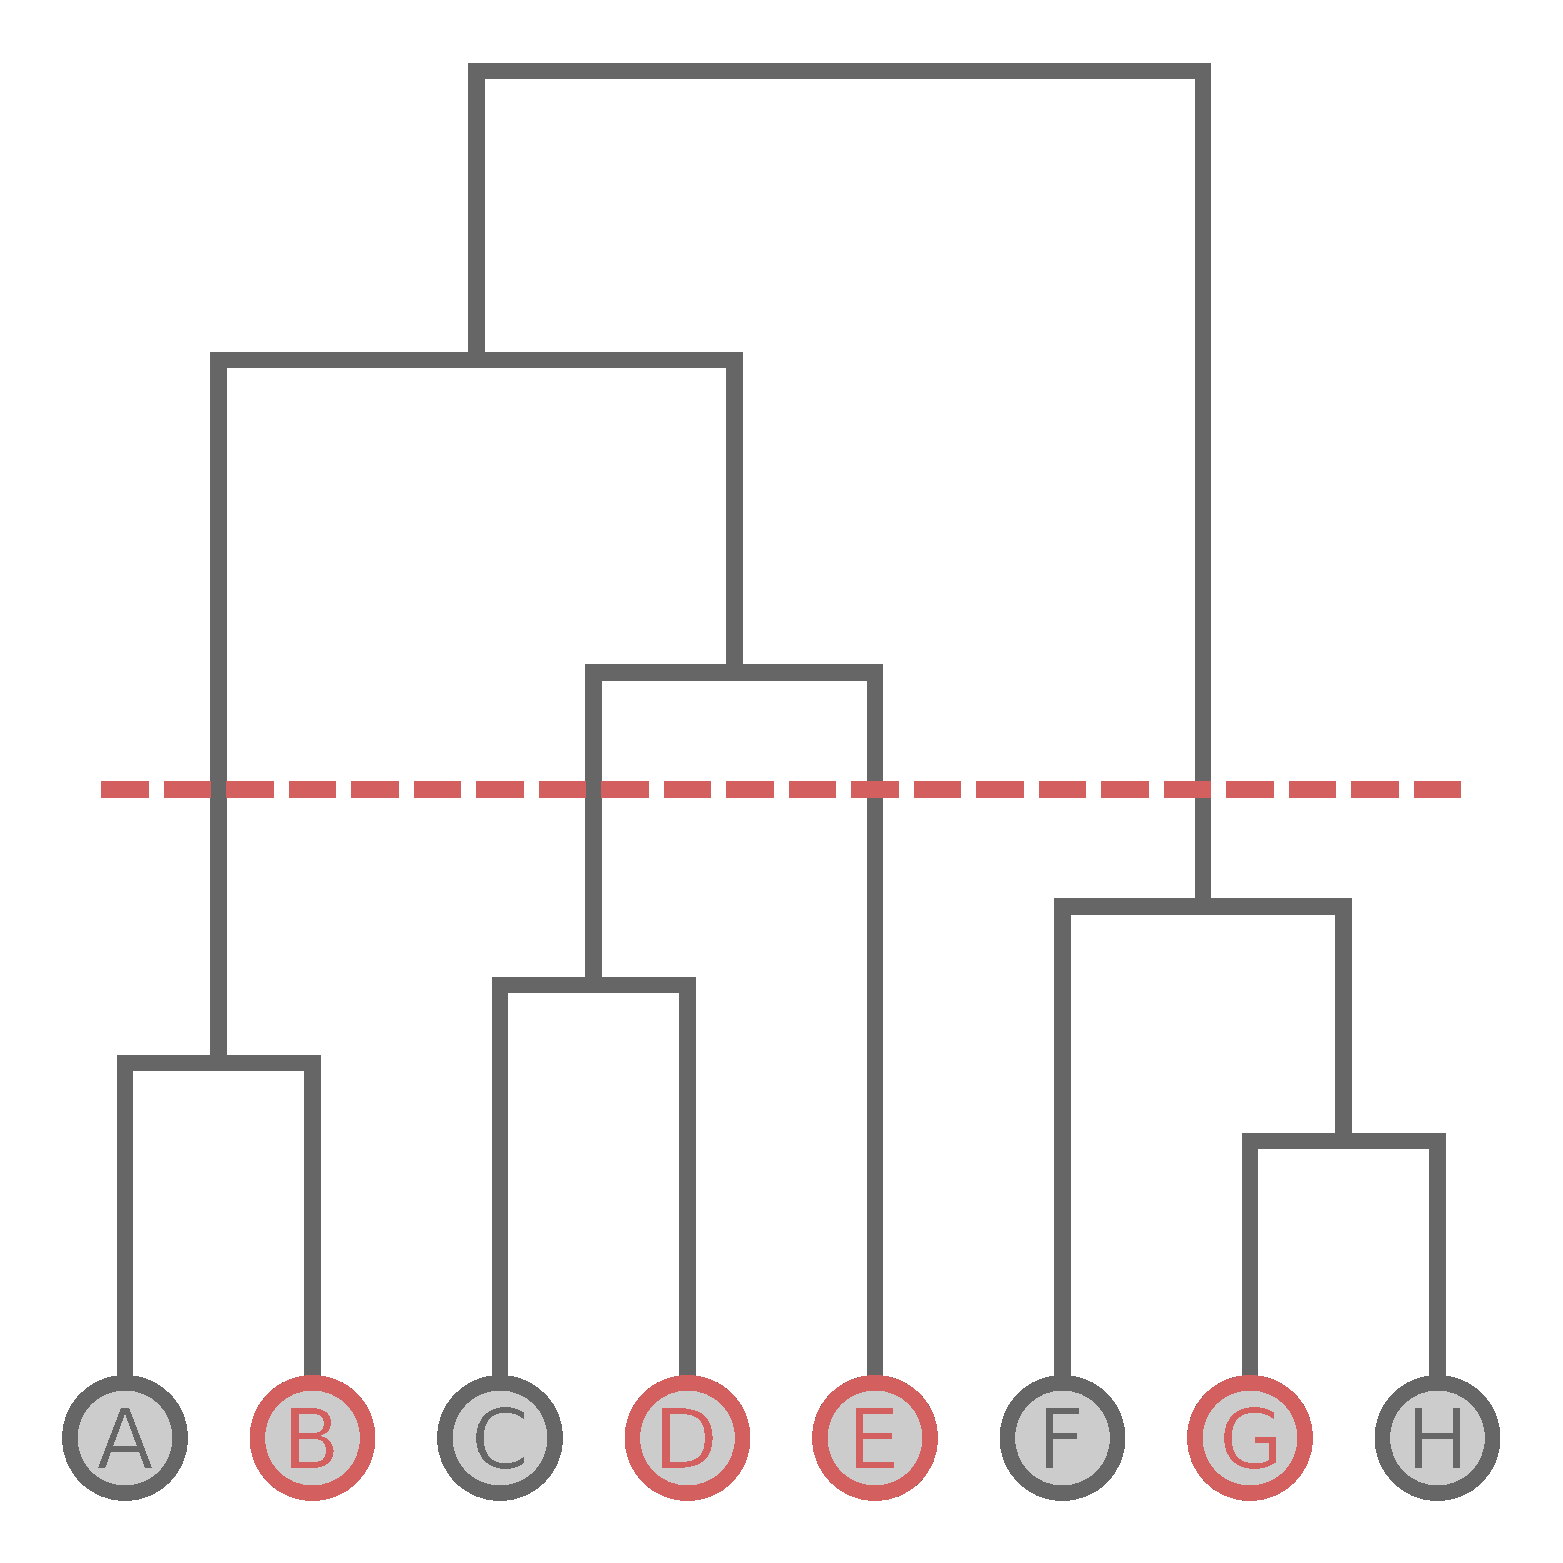
\includegraphics[width=\textwidth]{Graphics/Connectedness.pdf}
    \end{subfigure}
    %\end{adjustbox}
    \caption[Clustering Methods]{\textbf{Clustering Methods.} .}
    \label{fig:Methods}
\end{figure}

\section{WHO classification of \textit{Influenza A Virus}}

The present day classification of \gls{IAV} is based on the serotype of the virus 

\section{The proposed project}

%To increase the overall efficiency, strategies of next-generation vaccines focus on less variable structures of \gls{HA} and other \gls{IAV} proteins, namely \gls{NA}, \gls{M2} and the \glspl{NP} \autocite{wei_next-generation_2020}. Predicting the overall structure of the \gls{IAV} segments, that are crucial for the virus survival are, thus, essential for drug and vaccine creation against \gls{IAV} and still 


%expected are so und so viele based on the evol variation in dem nature paper wo es nur um H1 ging blabla 1-10 cluster pro subtype





% hierarchical clustering \autocite{gower_minimum_1969}. 

% \blindtext



% \blindtext

% \begin{figure}
%     \centering
%     %\begin{adjustbox}{minipage=\dimexpr\textwidth-2\fboxsep-2\fboxrule,fbox}
%     \begin{subfigure}[b]{0.475\textwidth}
%         \caption[Euclidean]{\textbf{Euclidean}}
%         \label{subfig:Euclidean}
%         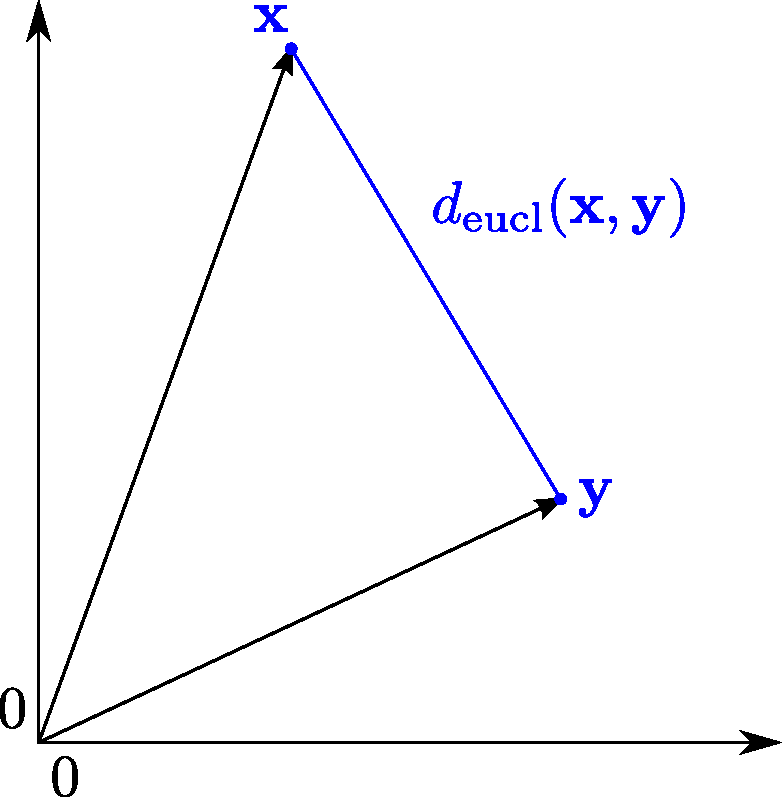
\includegraphics[width=\textwidth]{Graphics/Euclidean.pdf}
%     \end{subfigure}
%     \hfill
%     \begin{subfigure}[b]{0.475\textwidth}
%         \caption[Cosine]{\textbf{Cosine}}
%         \label{subfig:Cosinus}            
%         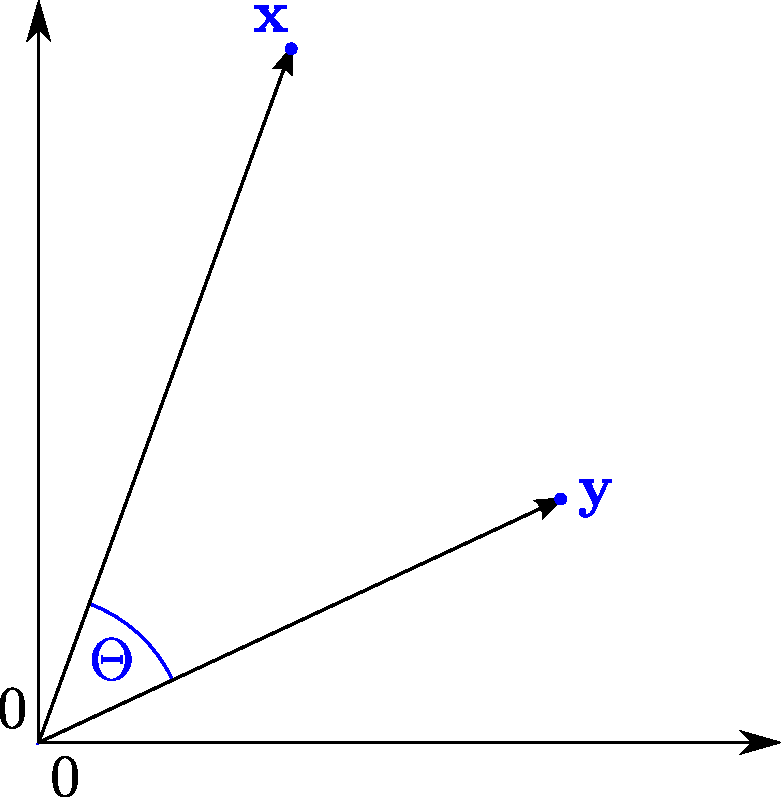
\includegraphics[width=\textwidth]{Graphics/Cosinus.pdf}
%     \end{subfigure}
%     %\end{adjustbox}
%     \caption[Distance Measuring Methods]{\textbf{Distance Measuring Methods.} .}
%     \label{fig:Distance}
% \end{figure}

% \blindtext

% % \begin{fequation}[!hbt]
% %     \begin{empheq}[box=\fbox]{alignat* = -1}
% %         &xL &&&&+zL &&\longrightarrow xL &&&&+zH\\
% %         &xM &&+yL &&+zH &&\longrightarrow xM &&+yL &&+zL\\
% %         &xM &&+yM &&+zL &&\longrightarrow xM &&+yM &&+zH\\
% %         &xH &&+yL &&+zH &&\longrightarrow xH &&+yL &&+zL\\
% %         &xH &&+yM &&+zH &&\longrightarrow xH &&+yM &&+zL\\
% %         & &&\hphantom{++}yH &&+zL &&\longrightarrow &&\hphantom{++}yH &&+zH
% %     \end{empheq}
% %     \caption[]{\textbf{.}}
% %     \label{gl:8.2}
% % \end{fequation}

% \textbf{Normalization with max-norm:} 
% %is the normalization so that the l2 norm of a vector is 1 !!!!!

% \begin{empheq}{alignat = -1}
%     \hat{\mathbf{x}} &= \frac{\mathbf{x}}{\Vert\mathbf{x}\Vert_{\text{max}}}
% \end{empheq}

% \begin{empheq}{alignat = -1}
%     \Vert\hat{\mathbf{x}}\Vert_{\text{max}} &= 1
% \end{empheq}

% \textbf{Cosinus similarity:}

% \begin{empheq}{alignat = -1}
%     %&\cos\angle(\mathbf{x}, \mathbf{y}) &&= \frac{\mathbf{x}^\top\mathbf{y}}{\Vert\mathbf{x}\Vert \cdot \Vert\mathbf{y}\Vert}
%     &\cos(\Theta) &&= \frac{\mathbf{x}^\top\mathbf{y}}{\Vert\mathbf{x}\Vert \cdot \Vert\mathbf{y}\Vert}
% \end{empheq}

% \textbf{cosinus distance}

% \begin{empheq}{alignat = -1}
%     %&d(\mathbf{x},\mathbf{y}) &&= 1 - \cos\angle(\mathbf{x}, \mathbf{y})
%     &d(\mathbf{x},\mathbf{y}) &&= 1 - \cos(\Theta)
% \end{empheq}

% \textbf{euclidean distance:}

% \begin{empheq}{alignat = -1}
%     &d(\mathbf{x},\mathbf{y}) &&= \Vert\mathbf{x} - \mathbf{y}\Vert_2
% \end{empheq}

% %gute anzahl cluster mit nennen 50-100 suoer bzw <100
% %außerdem erwartet, dass ansatzweise wie subtype bei H und N